\section{Building blocks of Latex writings}
This tex file contains the building bocks to write a paper.

\subsection{Tables}

\begin{table}[]
\tiny
\centering
\caption{Table 1}
\label{feedback-detail}
\begin{tabular}{|l|c|c|c|c|c|c|}
\hline
                   & \multicolumn{1}{l|}{\textbf{XXXX}} & \multicolumn{1}{l|}{\textbf{XXXX}} & \multicolumn{1}{l|}{\textbf{YYYY}} & \multicolumn{1}{l|}{\textbf{ZZZZ (\textless10 s)}} & \multicolumn{1}{l|}{\textbf{AAAA (\textgreater10s)}} & \multicolumn{1}{l|}{\textbf{BBB}} \\ \hline
\textbf{AAA}   & \textbf{66}   & \textbf{56}  & \textbf{76}  & \textbf{78}  & \textit{379} & \textit{785}  \\ \hline
\textbf{BBB} & \textit{161}  & \textit{117} & \textit{253} & \textit{521} & \textbf{192} & \textbf{218}  \\ \hline
%\textbf{Neutral}   & 201 & 59 & 177 & 292 & 197 & 254 \\ \hline
\end{tabular}
\end{table}


%\comment{ %omit-for-mobicom16
\begin{table} [ht]
\caption{Table 2}
\begin{center}
\setlength{\tabcolsep}{5pt}
%S\setlength{\extrarowheight}{1.5pt}
%\renewcommand{\arraystretch}{1.5}
%\begin{tabular}{|l|c|c|c|c|}
\begin{tabular}{|l|l|l|}
\hline
\bf{XX} &  \bf{YY} & \bf{ZZZ}\\
\hline
\hline
AAAAAAA & \bf{1} & \bf{0.326}\\
\hline
BBBBBBB & \bf{2} & \bf{0.226}\\
\hline
CCCCCCC & \bf{3} & \bf{0.204}\\
\hline
DDDDDDD & \bf{4} & \bf{0.201}\\
\hline
\end{tabular}
\end{center}
\label{table:feat_result}
\end{table}


\begin{table*} [ht]
\caption{This is a Two Column Long Table}
\begin{center}
\setlength{\tabcolsep}{5pt}
%S\setlength{\extrarowheight}{1.5pt}
\renewcommand{\arraystretch}{1.5}
%\begin{tabular}{|l|c|c|c|c|}
\begin{tabular}{|l||l|l|l|l|}
\hline
\bf{XXXXXXXXX} &  \bf{XXXXXXXX} & \bf{XXXXXXXX} & \bf{XXXXXXX} & \bf{XXXXXXXX}\\
\hline
\hline
YYYYYYYYYYYYYYYYYYY & 0.78 & 0.79 & 0.79 & 0.79 \\
\hline
YYYYYYYYYYYYYYYYYYY & \bf{0.95} & 0.96 & 0.96 & 0.96 \\
\hline
\end{tabular}
\end{center}
\label{table:class_result}
\end{table*}

\subsection{Enumerate}

This is two subsec.

\noindent \textbf{Summary of Insights}
\begin{enumerate}
    \item I1.
    \item I2.
    \item I3.
    \item I4.
\end{enumerate}

\subsection{Figures}

\begin{figure}[h!t]
%\vspace{-0.1in}
\center{
\fbox{\includegraphics[width=0.40\textwidth, keepaspectratio]{figs/setup.jpg}}
%\vspace{-0.1in}
\caption{{\small This is a custom shopping isle setup with our cart \textit{Konark}}}
%\vspace{-0.1in}
\label{fig:konark_setup}
}
\end{figure}
To summarize, we make the following contributions:
\begin{sitemize}
\item Contrib 1.
\item Contrib 2.
\item Contrib 3.
\end{sitemize}

\begin{figure}[hbt]
  \vspace{-0.15in}
\centering{
\subfigure[]{
    \fbox{\includegraphics[width=0.10\textwidth, keepaspectratio]{figs/dummy.png}}
    \label{fig:notifbase_front}
}
\subfigure[]{

    \fbox{\includegraphics[width=0.10\textwidth,  keepaspectratio]{figs/dummy.png}}
    \label{fig:notifbase_land}

}
\vspace{-0.15in}
\caption{{\small (a). Dummy Sub-Figure 1. (b). Dummy Sub-Figure 2 }}
%\vspace{-0.15in}
\label{fig:notifbase}
}
\end{figure}

\centering{
\subfigure[]{
    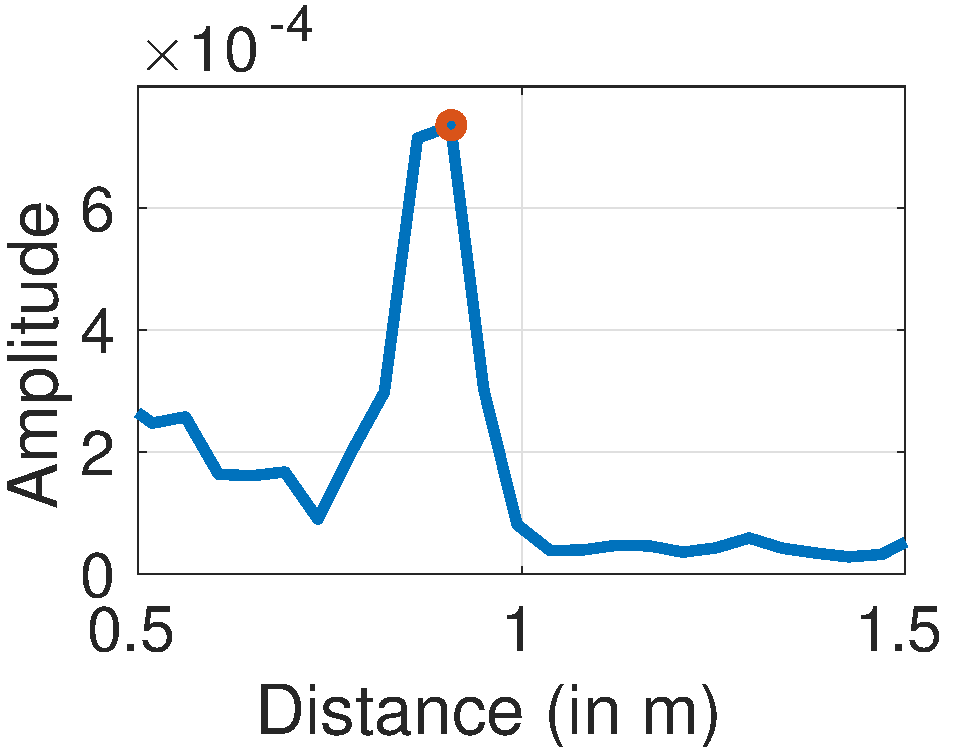
\includegraphics[width=0.10\textwidth, keepaspectratio]{figs/4K.pdf}
    \label{fig:4K}
}
\subfigure[]{

    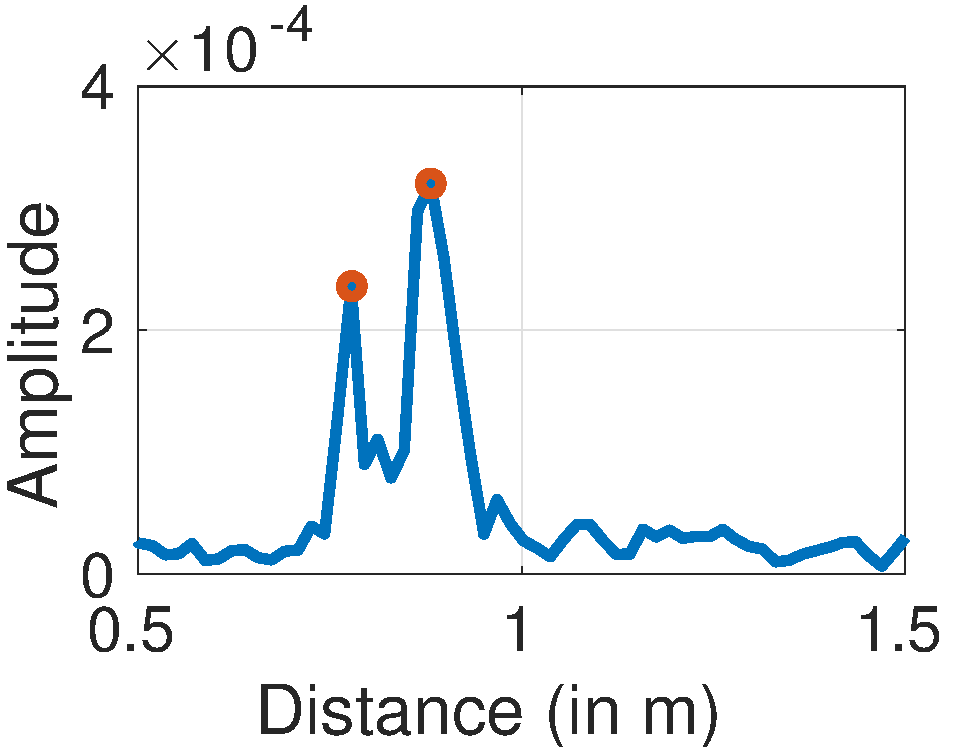
\includegraphics[width=0.10\textwidth,  keepaspectratio]{figs/10K.pdf}
    \label{fig:10K}

}
%\vspace{-0.15in}
\caption{{\small (a). 4KHz bandwidth used. (b). 10 KHz bandwidth used. }}
%\vspace{-0.15in}
\label{fig:resolution}
}
\end{figure}

\begin{figure}[h!t]
%\vspace{-0.1in}
\center{
\includegraphics[width=\columnwidth]{figs/dummy-pdf.pdf}
%\vspace{-0.1in}
\caption{{\small This is dummy figure}}
%\vspace{-0.1in}
\label{fig:res_prec_recall}
}
\end{figure}

